% ==============================================================================
% CAPÍTULO 5 - DESENVOLVIMENTO
% ==============================================================================

\chapter{Desenvolvimento}
\label{cap:desenvolvimento}

Este capítulo descreve o processo de análise, modelagem e implementação do módulo de geração
automatizada de propostas técnicas e comerciais (orçamentos) em PDF. O trabalho partiu do diagnóstico
do sistema legado, passou pela concepção de uma nova arquitetura orientada a layouts intercambiáveis e
chegou à implementação de um pipeline completo, do banco de dados à entrega do arquivo PDF ao
navegador.

%-------------------------------------------------
\section{Análise e Levantamento de Requisitos}
%-------------------------------------------------
\label{sec:requisitos}

O processo de levantamento de requisitos foi conduzido por meio de reuniões com o supervisor de estágio
e da análise direta do sistema existente. A inspeção do código legado revelou que a geração de
orçamentos era realizada pela função \texttt{generate\_orcamento}, localizada no módulo
\texttt{comercial/latex.py}, que utilizava a biblioteca PyLaTeX para construir o documento PDF
programaticamente, adicionando tabelas, seções e formatações por meio de chamadas de função Python.
Embora funcional, essa abordagem apresentava limitações estruturais relevantes:

\begin{alineas}
    \item O layout do documento estava \textbf{codificado diretamente no código Python}, impossibilitando
    alterações visuais sem intervenção de desenvolvedor;
    \item Não havia suporte a \textbf{múltiplos layouts}, qualquer nova identidade visual exigia a
    reescrita da função de geração;
    \item A inclusão de \textbf{descrições técnicas dos equipamentos} por conjunto (componente de
    produto) não era contemplada de forma sistemática, prejudicando a completude da proposta.
\end{alineas}

Simultaneamente, a empresa contratou uma empresa de design para elaborar um novo modelo visual de
proposta comercial. Esse layout foi entregue como referência visual (não como arquivo LaTeX), cabendo ao
estagiário a sua codificação no formato \texttt{.tex}.

A partir dessa análise, foram definidos os seguintes requisitos:

\textbf{Requisitos Funcionais:}
\begin{alineas}
    \item O sistema deve permitir o cadastro de layouts de orçamento via painel administrativo do Django,
    com upload do template compactado em formato \texttt{.zip};
    \item Apenas um layout pode estar ativo por vez; a ativação de um novo layout deve desativar
    automaticamente o anterior;
    \item A geração do PDF deve utilizar o layout ativo no momento da requisição, sem necessidade de
    configuração manual;
    \item O documento gerado deve incluir: informações cadastrais do cliente, tabela de equipamentos com
    valores, descrições técnicas por conjunto de produto, imagens dos equipamentos e condições comerciais;
    \item O sistema deve ser compatível com orçamentos contendo múltiplos equipamentos, cada um com sua
    própria composição de conjuntos e opcionais.
\end{alineas}

\textbf{Requisitos Não Funcionais:}
\begin{alineas}
    \item A solução deve ser implementada dentro do \textit{framework} Django, seguindo os padrões já
    estabelecidos no sistema da empresa;
    \item O template LaTeX deve ser processado pelo sistema de templates do Django, exigindo tratamento
    adequado dos conflitos de sintaxe entre os dois sistemas;
    \item O compilador utilizado deve ser o LuaLaTeX via \texttt{latexmk}, padrão já adotado em outros
    módulos do sistema;
    \item A troca de layout não deve exigir alterações no código-fonte da aplicação.
\end{alineas}

%-------------------------------------------------
\section{Modelagem}
%-------------------------------------------------
\label{sec:modelagem}

\subsection{Contexto dos Modelos Existentes}

O sistema comercial já possuía os seguintes modelos centrais para o processo de orçamento:

\begin{alineas}
    \item \texttt{Orcamento}: representa a proposta comercial, com número de série, cliente, vendedor,
    versão e status;
    \item \texttt{OrcamentoEquipamento}: representa cada item do orçamento, armazenando o campo
    \texttt{equipamentodetail} --- uma cadeia de códigos de conjuntos de produto separados por ponto, que
    define a composição técnica do equipamento;
    \item \texttt{OrcamentoCondicoes}: armazena as condições comerciais da proposta (prazo, frete,
    garantia, pagamento);
    \item \texttt{DescricaoOrcamento\_Conjunto}: associa conjuntos de produto a textos descritivos
    utilizados nas propostas, com suporte a prioridade e configuração de chave;
    \item \texttt{RegraImagem\_Conjunto}: associa conjuntos de produto a imagens representativas,
    utilizadas no documento.
\end{alineas}

Os dois últimos modelos são detalhados nas subseções a seguir, pois receberam extensões diretas
durante o desenvolvimento.

\subsubsection{Modelo DescricaoOrcamento\_Conjunto}

O modelo \texttt{DescricaoOrcamento\_Conjunto} já existia no sistema e é responsável por vincular
textos descritivos a conjuntos de produto. Cada registro associa um ou mais conjuntos (relação
muitos-para-muitos) a um identificador curto (\texttt{orcamento\_desc}), um texto longo opcional
(\texttt{description}), uma configuração de chave (\texttt{config\_chave}) e um campo de
prioridade para ordenação.

No contexto deste projeto, duas contribuições foram realizadas sobre esse modelo: a adição de
uma chave estrangeira opcional para \texttt{LayoutOrcamento}, permitindo vincular descrições a
um layout específico; e a implementação do método \texttt{atende\_conjuntos(codes\_item)}, que
verifica se o registro é aplicável a um dado equipamento, agrupa os conjuntos vinculados por
configuração e retorna verdadeiro somente se \texttt{codes\_item} possui interseção com todos os
grupos, garantindo que apenas descrições pertinentes ao equipamento sejam incluídas na proposta.
A \autoref{fig:modelo-descricao} ilustra a estrutura e a lógica do modelo.

\begin{figure}[htb]
    \caption{\label{fig:modelo-descricao}Estrutura e lógica do modelo \texttt{DescricaoOrcamento\_Conjunto}}
    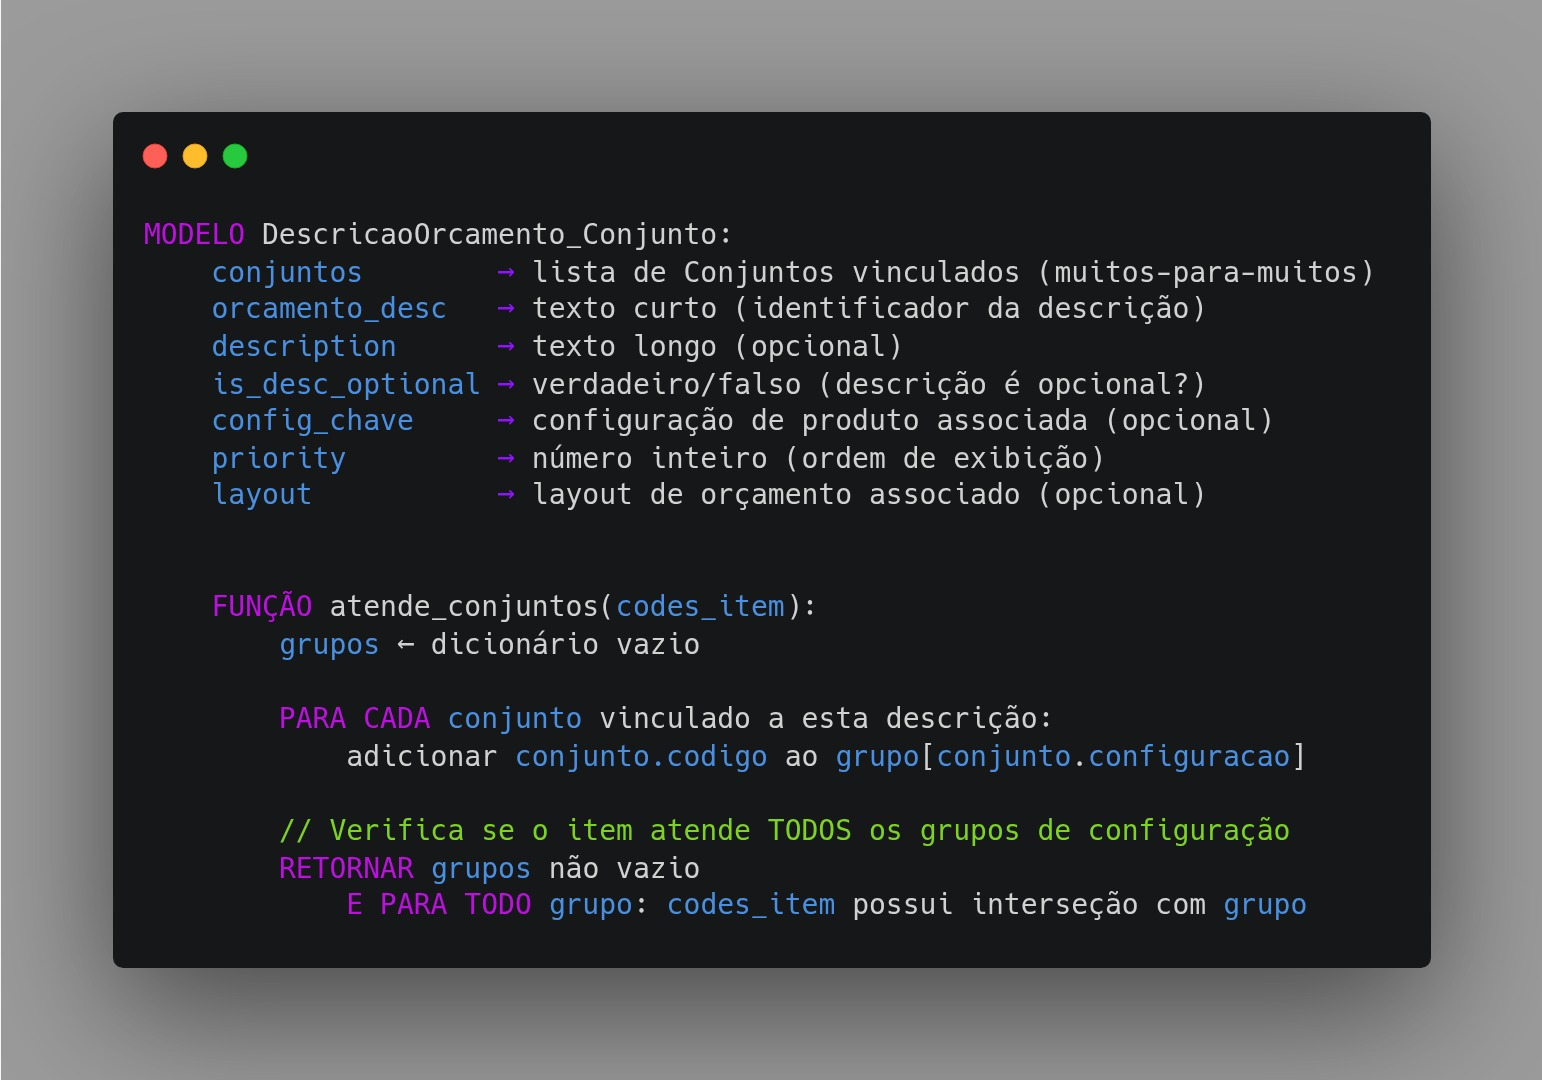
\includegraphics[width=0.85\textwidth]{figuras/05-desenvolvimento/Pseudo Código/Modelo descriçãoOrcamento_Conjunto.jpeg}
    \legend{Fonte: Própria do autor (2026), elaborado com Carbon (carbon.now.sh).}
\end{figure}

\subsubsection{Modelo RegraImagem\_Conjunto}

O modelo \texttt{RegraImagem\_Conjunto} segue estrutura análoga ao anterior, já existindo anteriormente, porém voltado
a imagens representativas dos equipamentos. Cada registro vincula um ou mais conjuntos ao
arquivo de imagem (\texttt{image}), a um identificador (\texttt{orcamento\_desc}) e a uma URL
opcional (\texttt{link}). O método \texttt{atende\_imagem(codes\_item)} aplica a mesma lógica
de interseção por grupos de configuração para determinar se a imagem é pertinente ao equipamento
em questão. A \autoref{fig:modelo-regraImagem} apresenta a estrutura do modelo.

\begin{figure}[htb]
    \caption{\label{fig:modelo-regraImagem}Estrutura e lógica do modelo \texttt{RegraImagem\_Conjunto}}
    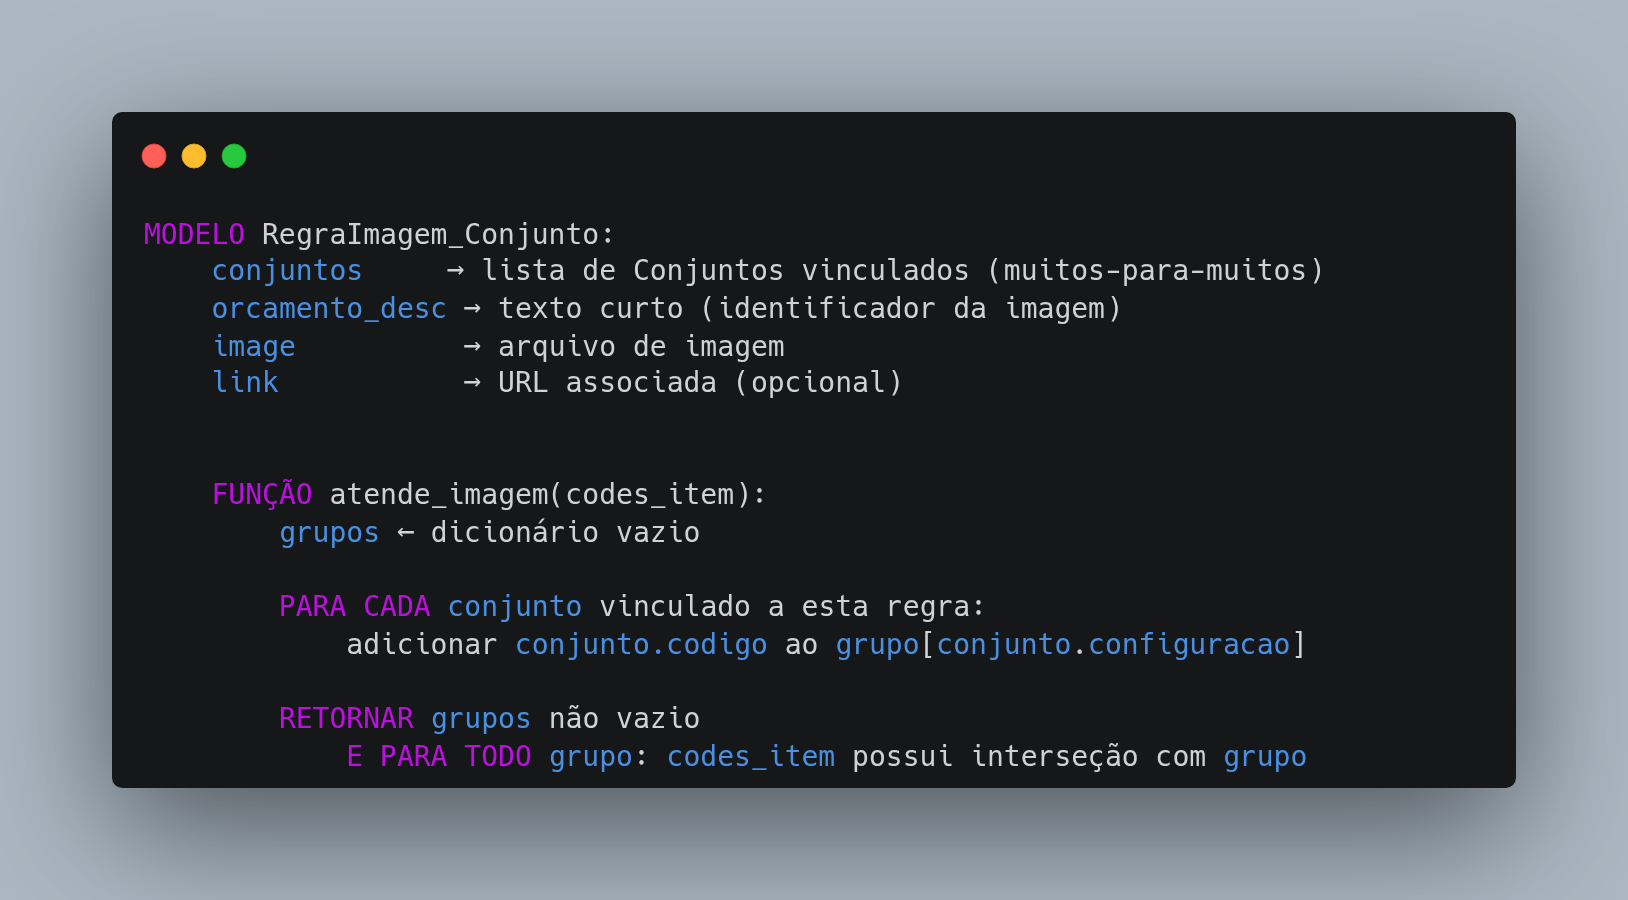
\includegraphics[width=0.85\textwidth]{figuras/05-desenvolvimento/Pseudo Código/ModeloRegraImagem.png}
    \legend{Fonte: Própria do autor (2026), elaborado com Carbon (carbon.now.sh).}
\end{figure}

\subsection{Novo Modelo: LayoutOrcamento}

Para suportar layouts intercambiáveis, foi projetado e implementado o modelo \texttt{LayoutOrcamento},
cuja estrutura é apresentada na \autoref{fig:modelo-layout} e detalhada no
Quadro~\ref{qdr:layout-orcamento}.

\begin{figure}[htb]
    \caption{\label{fig:modelo-layout}Estrutura e comportamento do modelo \texttt{LayoutOrcamento}}
    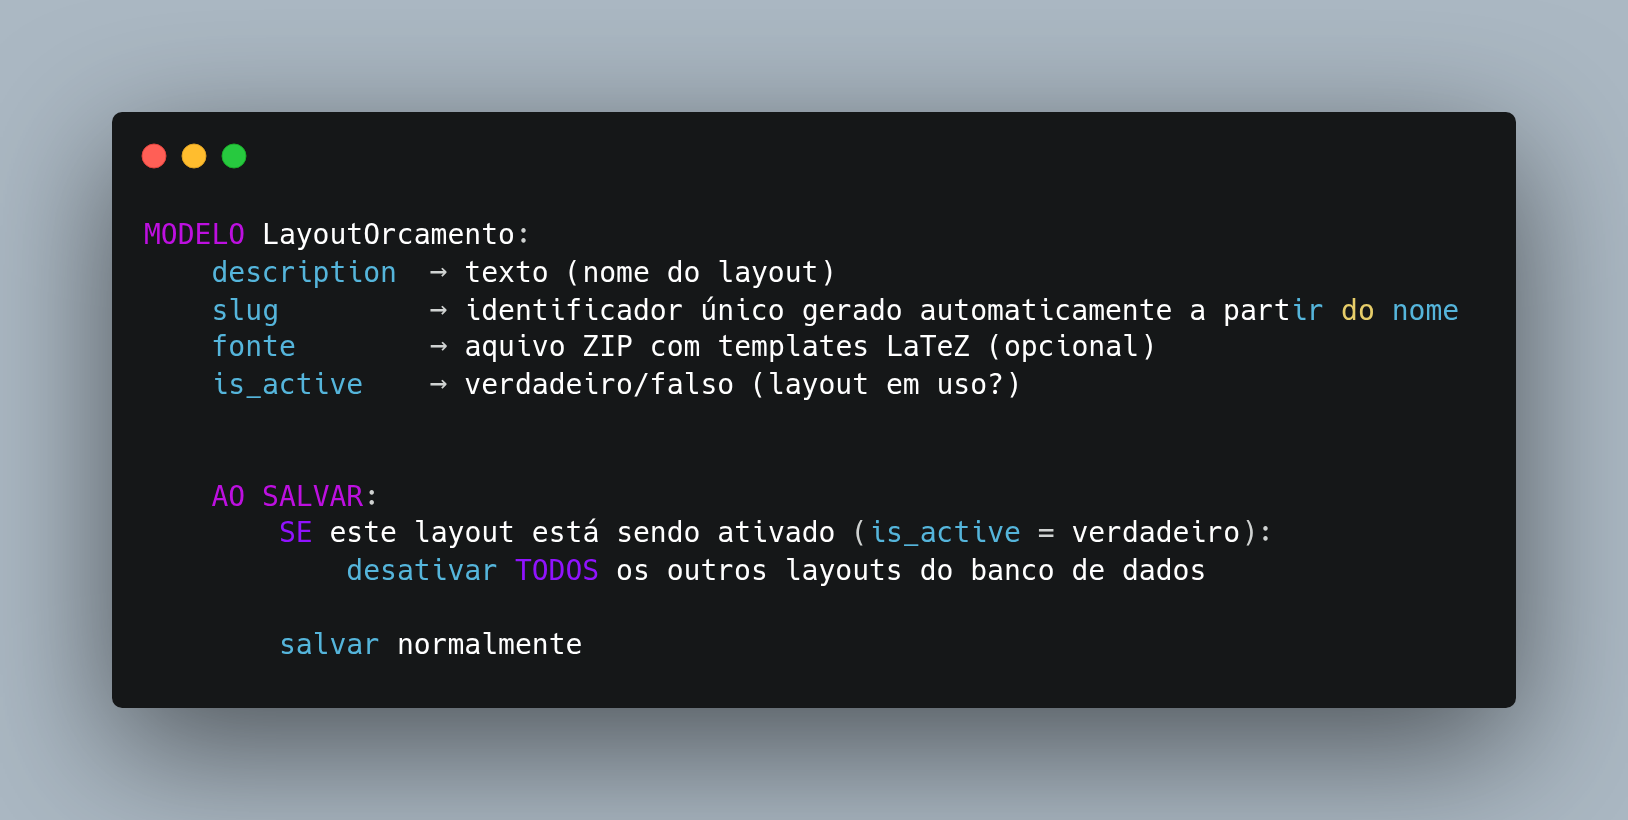
\includegraphics[width=0.75\textwidth]{figuras/05-desenvolvimento/Pseudo Código/ModeloLayoutOrcamento.png}
    \legend{Fonte: Própria do autor (2026), elaborado com Carbon (carbon.now.sh).}
\end{figure}

\begin{quadro}[htb]
    \caption{\label{qdr:layout-orcamento}Campos do modelo \texttt{LayoutOrcamento}}
    \begin{tabular}{|l|l|p{7cm}|}
        \hline
        \textbf{Campo} & \textbf{Tipo} & \textbf{Descrição} \\
        \hline
        \texttt{description} & \texttt{CharField} & Nome descritivo do layout \\
        \hline
        \texttt{slug} & \texttt{AutoSlugField} & Identificador único gerado a partir de \texttt{description} \\
        \hline
        \texttt{fonte} & \texttt{FileField} & Arquivo \texttt{.zip} contendo o template LaTeX e seus assets \\
        \hline
        \texttt{is\_active} & \texttt{BooleanField} & Indica se este é o layout em uso \\
        \hline
    \end{tabular}
    \legend{Fonte: Própria do autor (2026), elaborado com Carbon (carbon.now.sh).}
\end{quadro}

Uma decisão central de modelagem foi \textbf{não incluir} uma chave estrangeira de
\texttt{LayoutOrcamento} no modelo \texttt{Orcamento}. Essa escolha mantém o modelo de negócio
desacoplado das decisões de apresentação: o layout ativo é resolvido em tempo de geração,
por meio de uma consulta direta ao registro marcado como ativo, e não é persistido no orçamento.
Isso significa que diferentes gerações do mesmo orçamento podem utilizar layouts distintos,
conforme o layout ativo no momento --- comportamento adequado à realidade operacional da empresa,
onde a troca de layout é uma decisão de identidade visual global, não individual por proposta.

Os modelos \texttt{DescricaoOrcamento\_Conjunto} e \texttt{RegraImagem\_Conjunto} receberam
chaves estrangeiras opcionais para \texttt{LayoutOrcamento}, permitindo que descrições e imagens
sejam vinculadas a um layout específico. O sistema aplica um filtro com fallback: retorna registros
do layout ativo ou, na ausência, registros sem layout definido --- garantindo compatibilidade com
dados cadastrados antes da implementação do novo sistema.

O mecanismo de layout único ativo é garantido pelo método \texttt{save()} sobrescrito no modelo:
ao ativar um layout, todos os demais são automaticamente desativados antes da persistência do
registro, conforme ilustrado na \autoref{fig:modelo-layout}.

%-------------------------------------------------
\section{Implementação}
%-------------------------------------------------
\label{sec:implementacao}

A implementação foi dividida em três frentes interdependentes: (a) a codificação do template LaTeX;
(b) o desenvolvimento das funções de suporte na \textit{view}; e (c) a integração do pipeline completo
de geração de PDF.

\subsection{Codificação do Template LaTeX}

O layout visual elaborado pela empresa de design foi traduzido para um arquivo \texttt{main.tex}
estruturado para ser processado pelo sistema de templates do Django. Esse processo exigiu atenção
especial ao \textbf{conflito de delimitadores} entre os dois sistemas: o LaTeX utiliza extensivamente
o caractere de percentual como início de comentário e chaves como delimitadores de argumentos de
comandos, enquanto o Django utiliza chaves duplas para variáveis e blocos percentual-chave para
\textit{tags} de controle.

A solução adotada, já consolidada em outros módulos do sistema, como \texttt{viewsinspecao.py},
consiste em configurar o motor de templates com delimitadores customizados, substituindo a sintaxe
padrão do Django por sequências que não colidem com a gramática do LaTeX. Essa abordagem permite que
o arquivo \texttt{.tex} seja ao mesmo tempo um template Django válido e um documento LaTeX
sintaticamente correto.

O template é organizado em seções que correspondem às partes visuais do documento:

\begin{alineas}
    \item \textbf{Cabeçalho}: logotipo da empresa e identificação da proposta;
    \item \textbf{Informações cadastrais}: dados do cliente (razão social, CNPJ, município, contato);
    \item \textbf{Tabela de equipamentos}: itens do orçamento com quantidade, valor unitário e
    valor total;
    \item \textbf{Descrições técnicas}: para cada equipamento, as descrições dos conjuntos que o
    compõem são listadas em formato de tabela com identificadores de atributo e valores;
    \item \textbf{Imagens dos equipamentos}: imagens associadas aos conjuntos via
    \texttt{RegraImagem\_Conjunto};
    \item \textbf{Condições de fornecimento}: pagamento, frete, garantia, prazo e serviços inclusos;
    \item \textbf{Rodapé}: dados de contato e assinatura do consultor.
\end{alineas}

\begin{figure}[htb]
    \caption{\label{fig:modelo-regraImagem}Estrutura e lógica do template \texttt{main.tex}}
    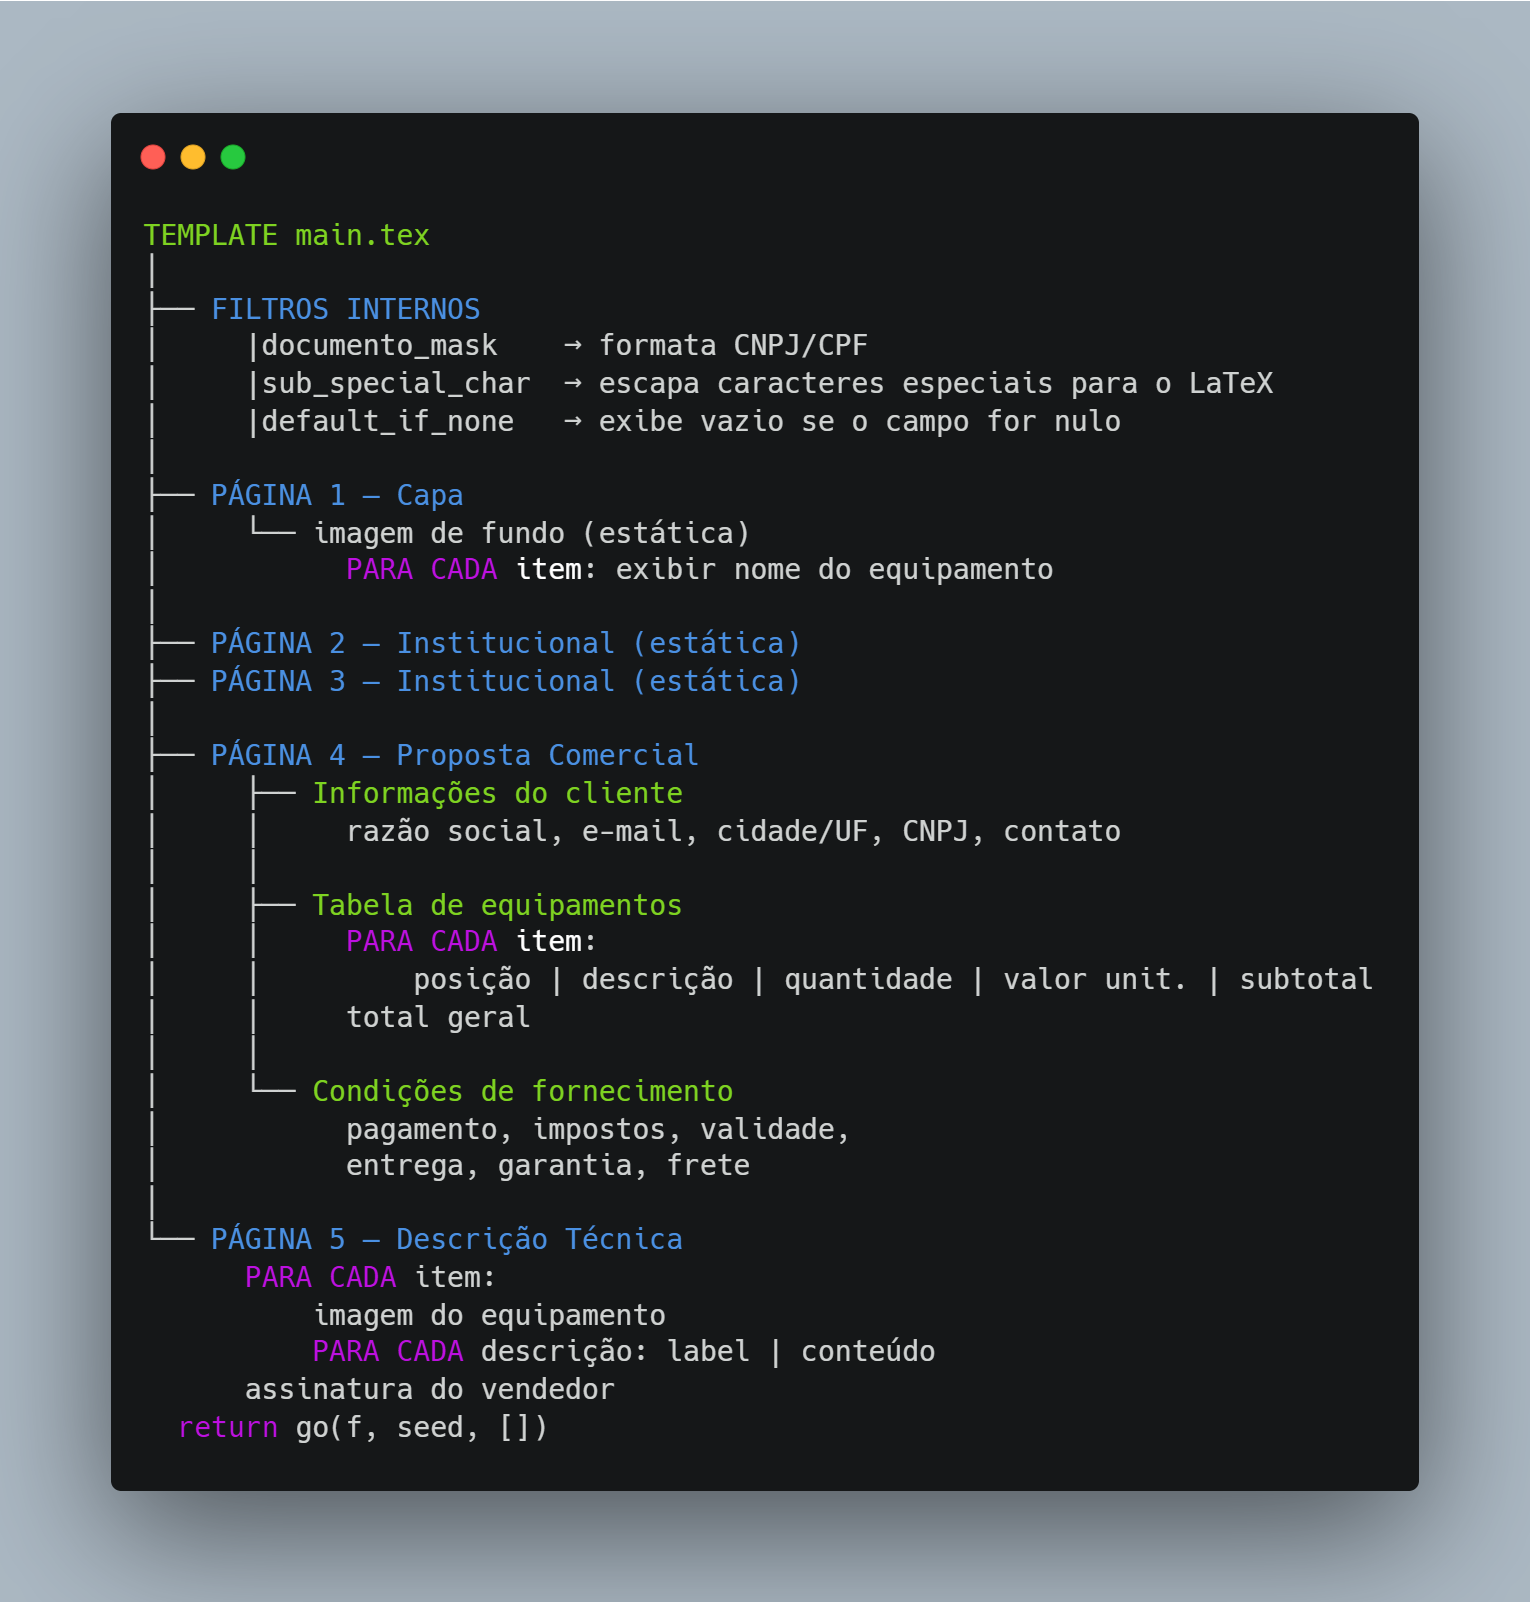
\includegraphics[width=0.85\textwidth]{figuras/05-desenvolvimento/Pseudo Código/TEX.png}
    \legend{Fonte: Própria do autor (2026), elaborado com Carbon (carbon.now.sh).}
\end{figure}

\subsection{Funções da \textit{View}}

Na camada de \textit{views}, foram implementadas três funções principais que compõem o pipeline de
geração, descritas a seguir.

\subsubsection{Função montar\_contexto\_orcamento\_layout}

A função \texttt{montar\_contexto\_orcamento\_layout} é responsável por construir o dicionário de
dados que será injetado no template LaTeX. Recebe o orçamento e a versão como parâmetros e,
internamente, resolve o layout ativo, as condições comerciais e os equipamentos vinculados ao
orçamento. Para cada equipamento, os códigos de conjuntos são extraídos do campo
\texttt{equipamentodetail} e utilizados para filtrar as descrições e imagens aplicáveis, por meio
dos métodos \texttt{atende\_conjuntos} e \texttt{atende\_imagem} descritos anteriormente.
As descrições são pré-carregadas com filtro de fallback --- layout ativo ou sem layout definido ---
e ordenadas por prioridade. O contexto retornado contém todos os dados necessários para a
renderização completa do documento, sem lógica de apresentação embutida.
A \autoref{fig:funcao-contexto} apresenta o pseudocódigo da função.

\begin{figure}[htb]
    \caption{\label{fig:funcao-contexto}Estrutura e lógica da função \texttt{montar\_contexto\_orcamento\_layout}}
    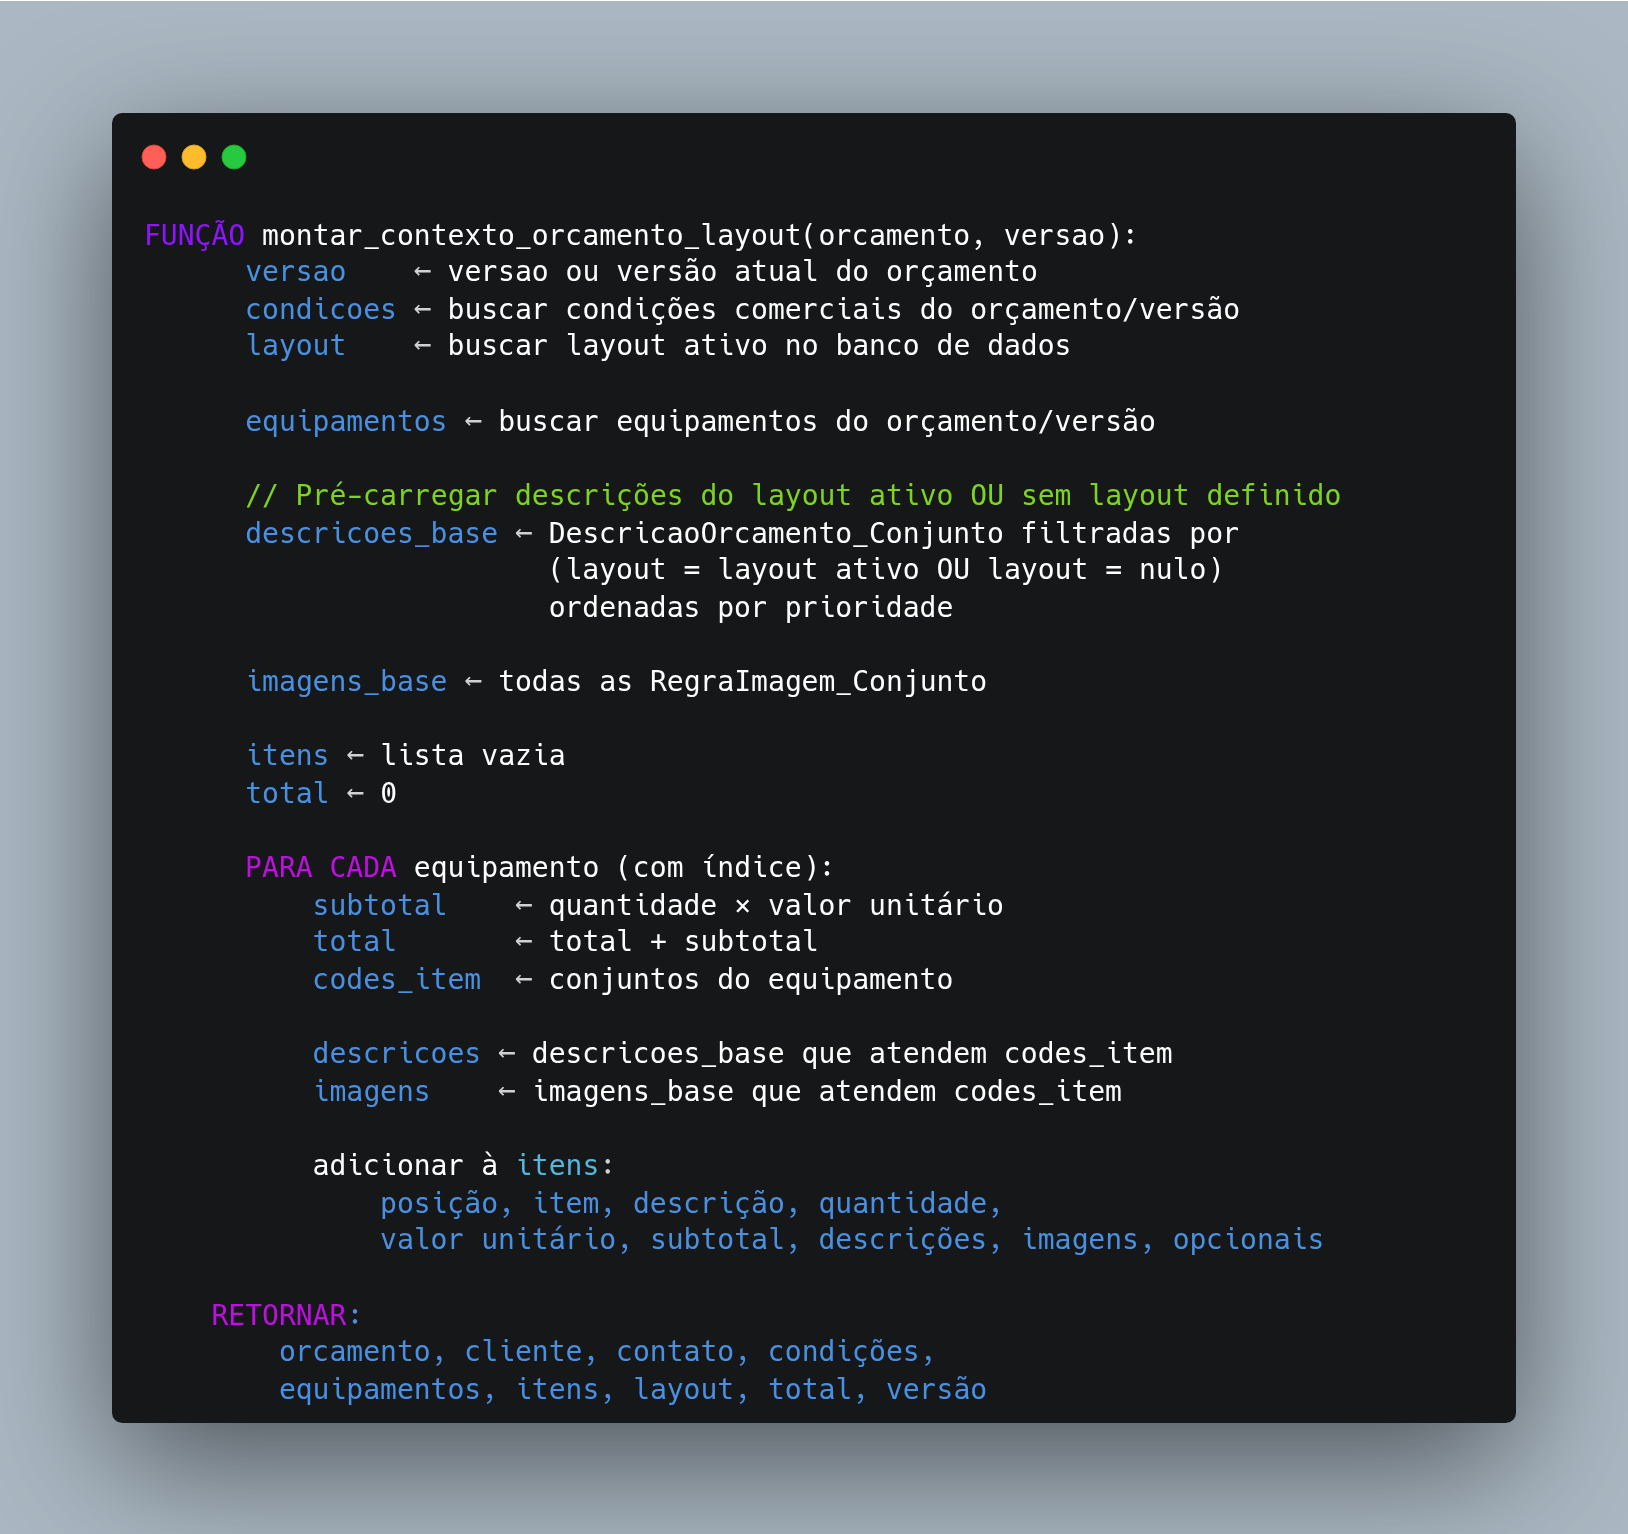
\includegraphics[width=0.90\textwidth]{figuras/05-desenvolvimento/Pseudo Código/funçãomontarcontexto.png}
    \legend{Fonte: Própria do autor (2026), elaborado com Carbon (carbon.now.sh).}
\end{figure}

\subsubsection{Função orcamento\_layout\_pdf\_view}

A função \texttt{orcamento\_layout\_pdf\_view} é a \textit{view} principal, responsável por
orquestrar todo o pipeline de geração. Recebe a requisição HTTP, o identificador do orçamento e
a versão, e executa a seguinte sequência: localiza o orçamento no banco de dados; resolve o layout
ativo e o diretório de trabalho do template; monta o contexto de dados; renderiza o template
\texttt{main.tex} com as variáveis substituídas; salva o arquivo \texttt{.tex} renderizado em disco;
aciona o compilador LuaLaTeX via \texttt{latexmk}; e retorna o PDF gerado como resposta HTTP.
Cada etapa possui tratamento de erro individual: ausência de layout ativo, arquivo ZIP não
encontrado, template ausente ou falha na compilação resultam em resposta 404 com registro do
erro no terminal. A \autoref{fig:funcao-view} apresenta o pseudocódigo da função.

\begin{figure}[htb]
    \caption{\label{fig:funcao-view}Estrutura e lógica da função \texttt{orcamento\_layout\_pdf\_view}}
    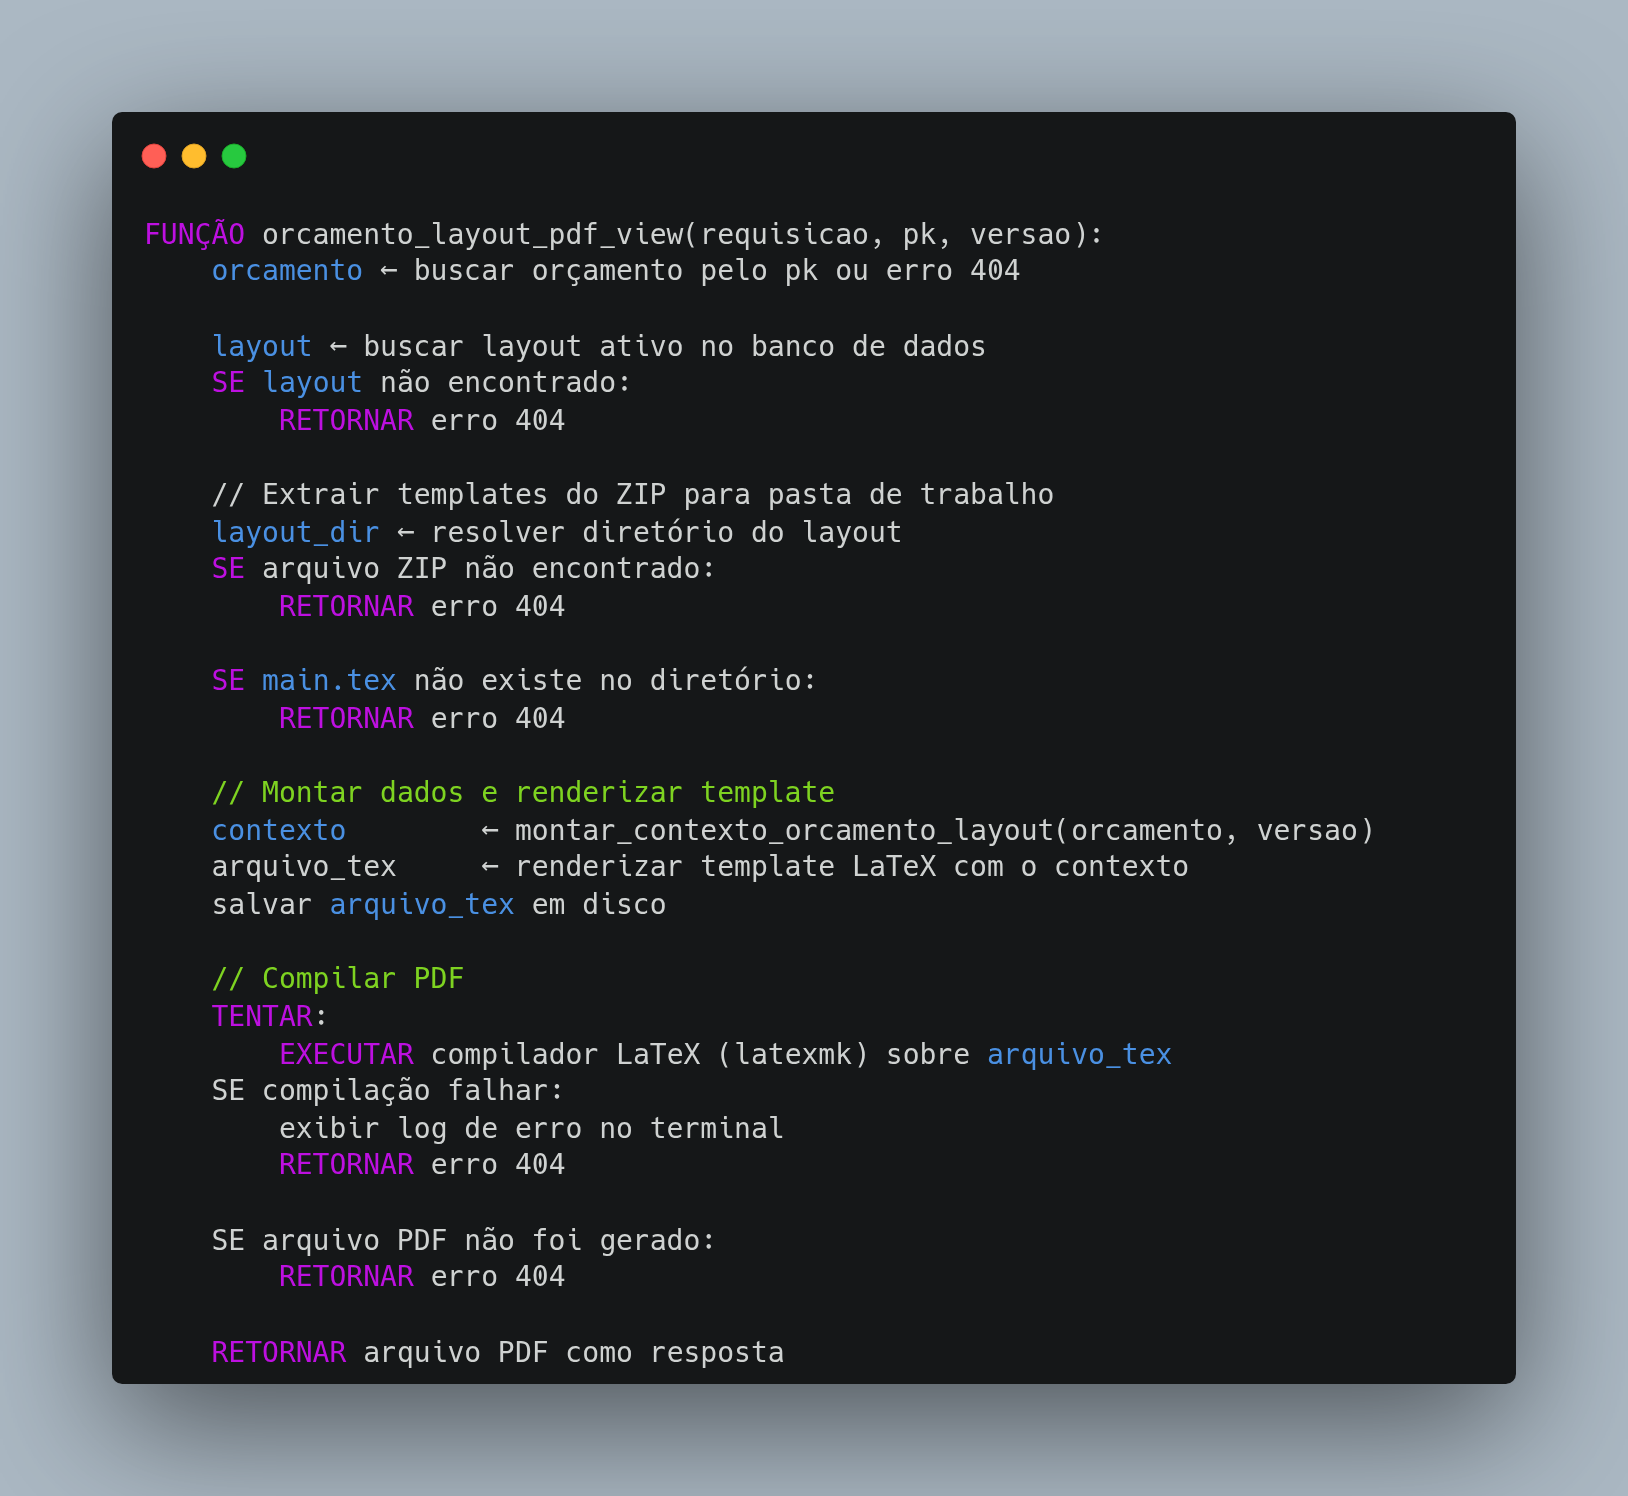
\includegraphics[width=0.90\textwidth]{figuras/05-desenvolvimento/Pseudo Código/FunçãoOrcamento_layout_pdf_view.png}
    \legend{Fonte: Própria do autor (2026), elaborado com Carbon (carbon.now.sh).}
\end{figure}

\subsection{Integração com o Django Admin}

O modelo \texttt{LayoutOrcamento} foi registrado no painel administrativo do Django, permitindo que
gestores realizem o upload de novos templates (\texttt{.zip}) e ativem um layout diretamente pela
interface web, sem qualquer interação com o código-fonte. Ao marcar o campo \texttt{is\_active}
como verdadeiro em um registro, o método \texttt{save()} sobrescrito desativa automaticamente
todos os demais layouts antes de salvar, garantindo a consistência do estado ativo único.

%-------------------------------------------------
\section{Resultados e Discussões}
%-------------------------------------------------
\label{sec:resultados}

Ao final do período de estágio, o pipeline de geração de orçamentos com o novo layout estava funcional
em ambiente de desenvolvimento: o template LaTeX era renderizado corretamente pelo sistema de templates
do Django e compilado com sucesso pelo \texttt{latexmk}, produzindo o PDF com o layout definido pela
empresa de design. A injeção das variáveis de contexto, dados do cliente, itens, descrições técnicas
e condições comerciais, estava em fase de validação final antes da integração ao ambiente de produção.

O Quadro~\ref{qdr:comparativo} apresenta uma comparação entre o sistema legado (PyLaTeX) e a nova
arquitetura implementada.

\begin{quadro}[htb]
    \caption{\label{qdr:comparativo}Comparativo entre o sistema legado e o sistema desenvolvido}
    \begin{tabular}{|p{4.5cm}|p{4.5cm}|p{4.5cm}|}
        \hline
        \textbf{Aspecto} & \textbf{Sistema Legado (PyLaTeX)} & \textbf{Novo Sistema (Django + \LaTeX)} \\
        \hline
        Alteração de layout & Requer modificação de código Python & Realizada via painel administrativo \\
        \hline
        Suporte a múltiplos layouts & Não & Sim, com ativação dinâmica \\
        \hline
        Descrições técnicas por conjunto & Não estruturado & Gerenciadas via modelo dedicado \\
        \hline
        Qualidade tipográfica & Limitada pela abstração da biblioteca PyLaTeX & Total controle via \LaTeX{} nativo \\
        \hline
        Separação de responsabilidades & Baixa (layout no código) & Alta (layout no template) \\
        \hline
    \end{tabular}
    \legend{Fonte: Própria do autor (2026).}
\end{quadro}

A decisão arquitetural de resolver o layout em tempo de geração --- em vez de persistir a referência
no modelo \texttt{Orcamento} --- mostrou-se adequada: manteve o modelo de negócio limpo e permitiu
que a troca de layout afete todas as gerações futuras sem exigir alterações em registros históricos.
A principal ressalva é que orçamentos gerados em momentos diferentes poderão ter layouts distintos,
o que é aceitável no contexto operacional da empresa e pode ser tratado futuramente com o
armazenamento do PDF gerado associado ao registro do orçamento.

O tratamento do conflito de delimitadores entre Django e \LaTeX{}, validado pela referência ao padrão
já utilizado no módulo de inspeção (\texttt{viewsinspecao.py}), demonstrou que a solução é extensível
a qualquer template \LaTeX{} processado pelo sistema, consolidando um padrão técnico reaproveitável
por toda a aplicação.